\documentclass[tikz,border=4pt]{standalone}
\begin{document}
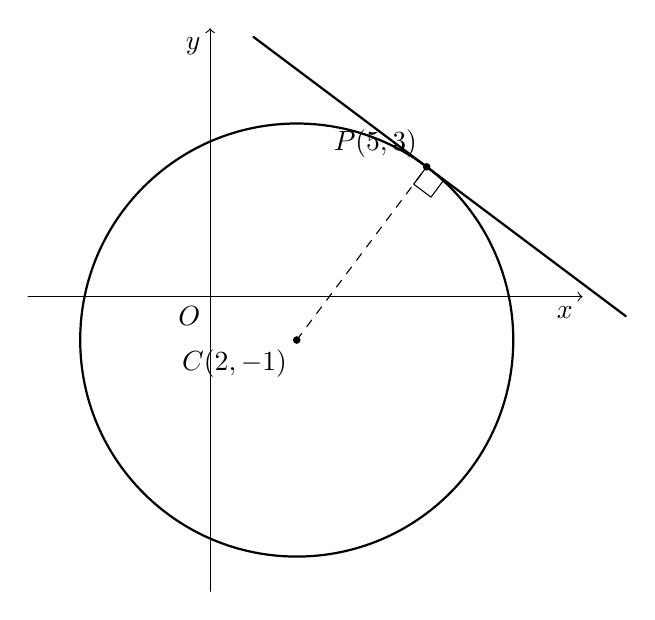
\begin{tikzpicture}[scale=0.55, line cap=round, line join=round]
  % sumbu
  \draw[->, thin] (-4.2,0) -- (8.6,0) node[below left] {$x$};
  \draw[->, thin] (0,-6.8) -- (0,6.2) node[below left] {$y$};
  \node[below left] at (0,0) {$O$};
  % lingkaran pusat (2,-1), jari-jari 5
  \draw[thick] (2,-1) circle (5);
  % garis singgung 3x+4y=27 di titik (5,3)
  \draw[thick] (1,6) -- (9.6,-0.45);
  % jari-jari ke titik singgung + tanda siku
  \draw[dashed] (2,-1) -- (5,3);
  \draw (5,3) -- (4.7,2.6) -- (5.1,2.3) -- (5.4,2.7);
  \fill (2,-1) circle (2.5pt) node[below left] {$C(2,-1)$};
  \fill (5,3) circle (2.5pt) node[above left] {$P(5,3)$};
\end{tikzpicture}
\end{document}
